\section{markdown conversion test}

\subsection{Header 1}
\textbf{Bold text}
small image:

\begin{center}
	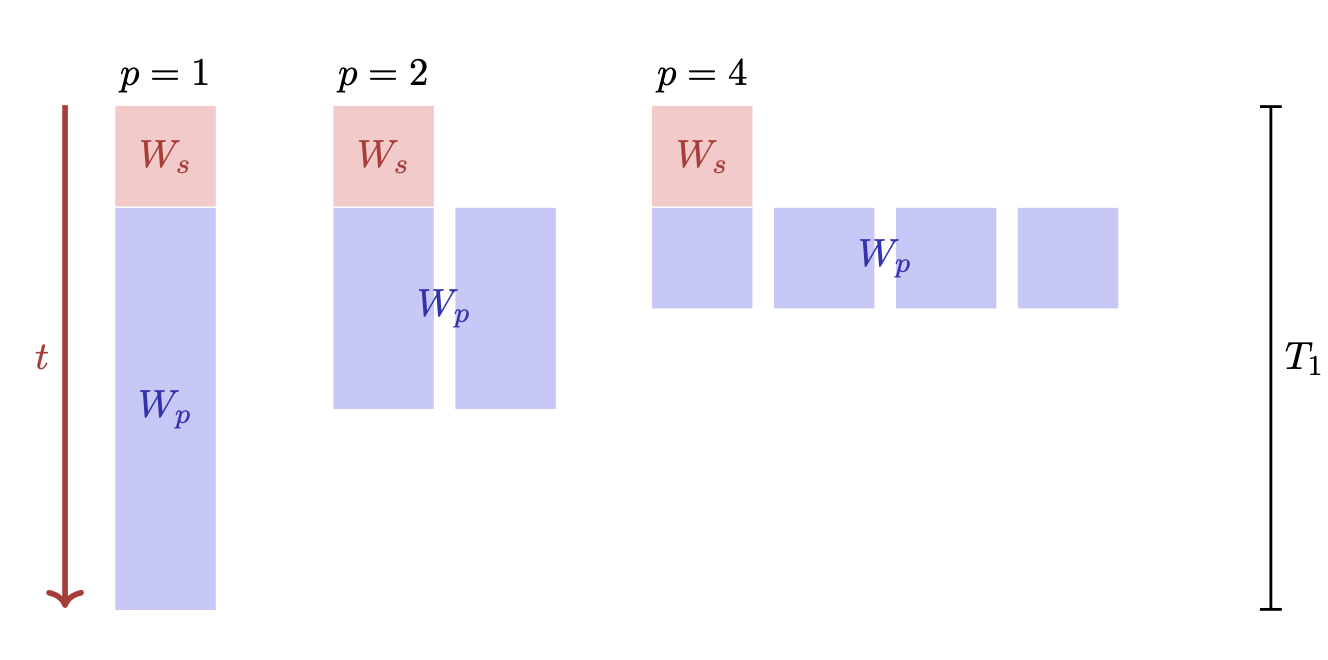
\includegraphics[width=0.7\linewidth]{amdahl.png}
\end{center}
medium image:

\begin{center}
	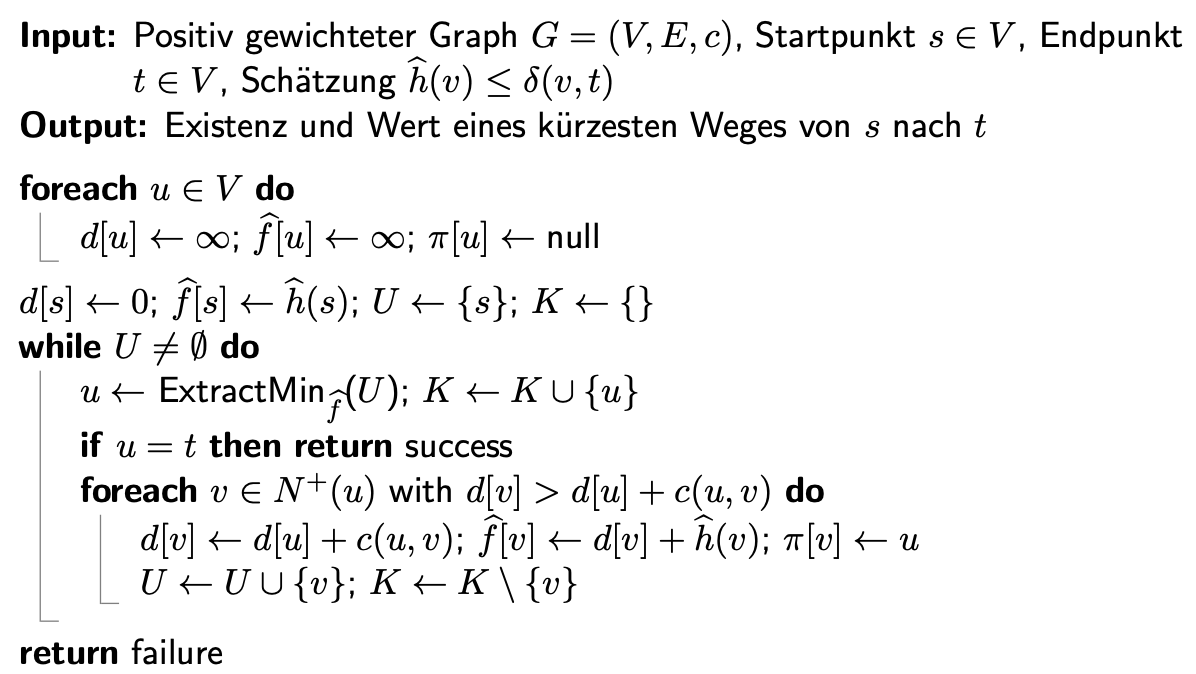
\includegraphics[width=0.9\linewidth]{astar.png}
\end{center}
large image

\begin{center}
	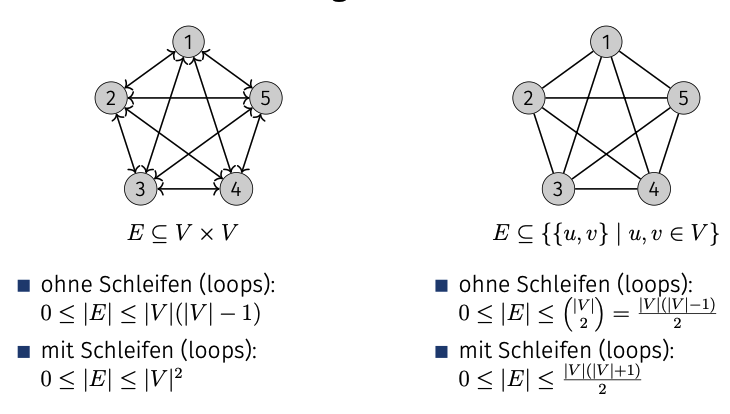
\includegraphics[width=\linewidth]{Beziehung_EV.png}
\end{center}

\subsubsection{Header 2}
\textit{Cursive Text}
\texttt{code line}

\lstset{style=bright}\begin{lstlisting}[basicstyle=\footnotesize, language=C++]
C++
Code Block
\end{lstlisting}

\begin{itemize}[leftmargin=8pt, label = ·]
	\item items
	\item items
\end{itemize}

> indent


\begin{enumerate}[leftmargin=12pt]
	\item first
	\item second
	\item third
\end{enumerate}


\paragraph{Header 3}
Text


\begin{equation*}
P=NP
\end{equation*}

\begin{align*}
 x&= 34\\
 y(t) &= 42
\end{align*}

